\begin{document}
\sectiontitle{5}{Software Refactoring}
\setstretch{1.6}

As mentioned introduction wise, this project builds upon the work and code base originally developed for the LegoPress \cite{olivier_legopress_2014} in C++ using Qt which was later expanded upon by a previous student. However, the code had become difficult to manage and the code quality poor, with thousands of lines of and multiple functionalities implemented in a single file and class. Therefore, before continuing on with the project a full refactoring of the code was necessary. The objective was to save time in the long run by creating modular, robust, readable code that could later be further developed and possibly used in clinical trials.

\subsection{Methods}
\begin{figure} [h]
	\centering
	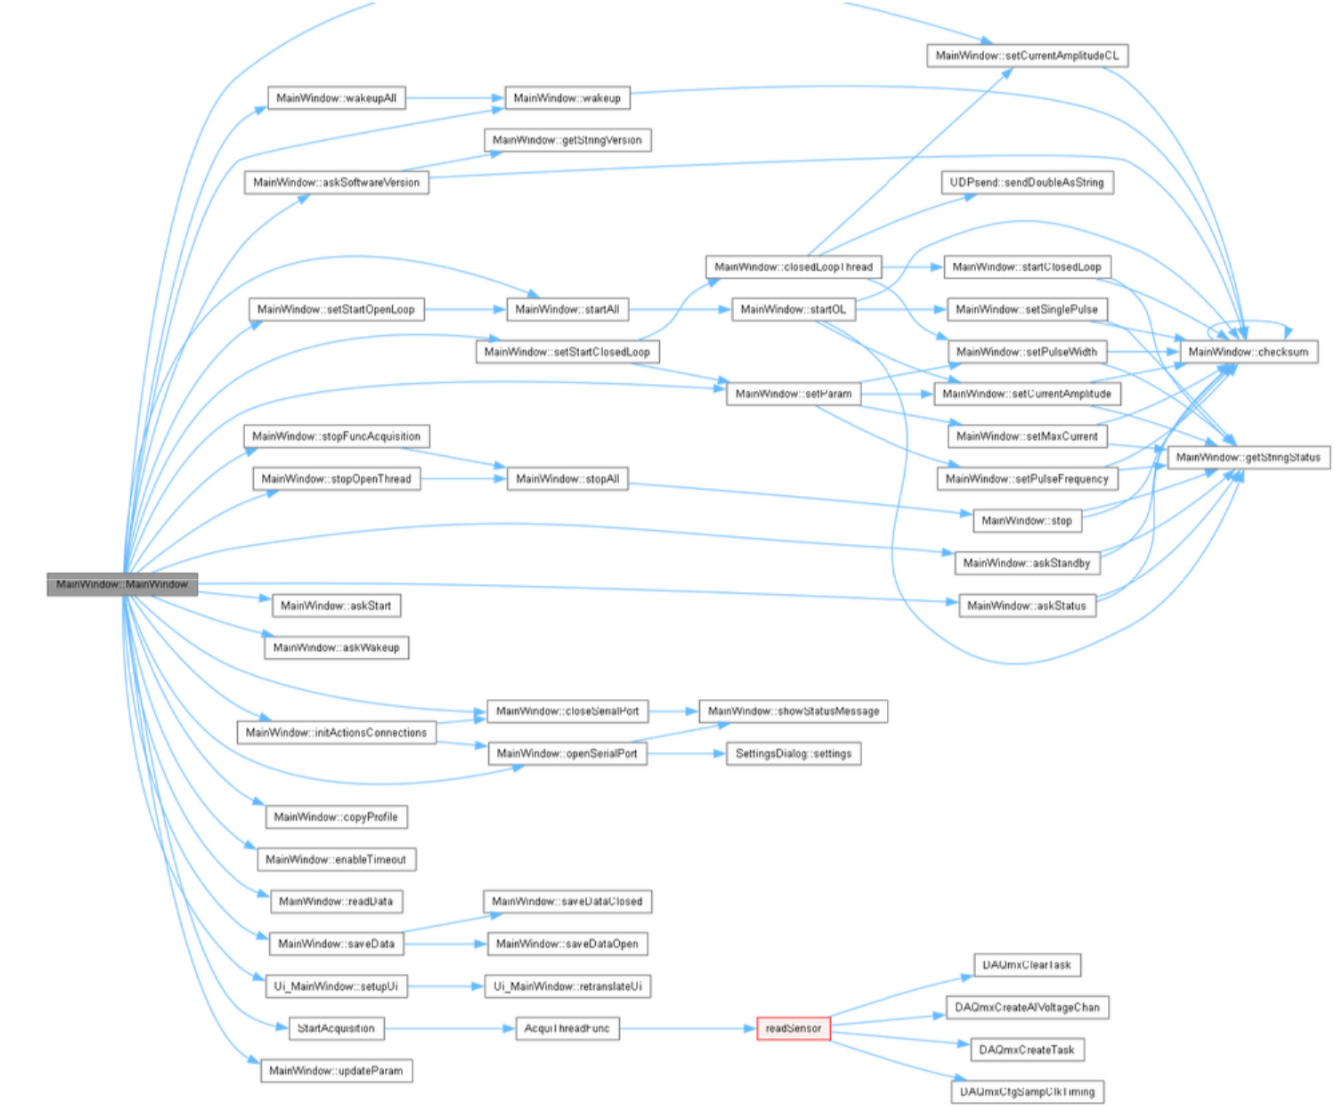
\includegraphics[width=0.9\linewidth]{images/oldDoxy.png}
	\caption{Doxygen-generated call graph for the original mainWindow function before refactoring}
	\label{fig:oldDoxy}
\end{figure}

To understand the code and its functionality, the first step was to document it. This involved editing the code to make it compatible with Doxygen, a tool that automatically generates software documentation in HTML or LaTeX from annotated source code \cite{noauthor_doxygen_nodate}. This includes graphical representations of call graphs, such as the one in figure \ref{fig:oldDoxy}, and hierarchies. These visualizations are particularly useful for analyzing the structure and functionality of an unfamiliar codebase, aiding the refactoring and modularization.

In order to improve the code quality, modularization and removal of irrelevant functionality was necessary. The code was refactored and divided into classes based on the code quality principles laid out in Code Complete by Steve McConnell \cite{steve_mcconnell_code_nodate}. This includes having clearly defined, minimal interfaces. Another core concept followed in the modularization is organizing modules hierarchically, where higher-level modules depend on lower-level modules but not the reverse, thereby avoiding circular dependencies. 

\subsection{Implementation}
The refactoring divided the code into seven distinct classes. Previously, all loop controller, IMU functionality, serial communication and bit handling was done in the \texttt{mainwindow} class. There was also legacy code from the LegoPress, completely irrelevant to this project, which was removed. Since this project involved the changing out of the previously utilized wired IMUs with new wireless IMUs, all the code relating to IMU functionality was also removed. The remaining functional code was moved to appropriate classes. These classes are: \texttt{MessageHandler}, \texttt{LoopController} and \texttt{MainWindow}. Additional classes were also added for the new functionality implemented during the project.

To ensure a clean and modular structure, the refactored design leveraged the signal-slot mechanism provided by Qt. This approach enabled event-driven, decoupled communication between objects, ensuring minimal and clearly defined interfaces across the newly organized classes.

\subsection{Results}
\begin{figure} [h]
    \centering
    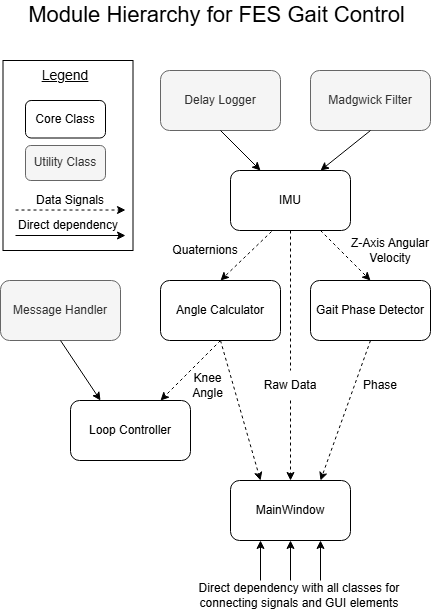
\includegraphics[width=0.6\linewidth]{images/gaitcontrol.png}
    \caption{Module hierarchy after refactoring}
    \label{fig:modulehier}
\end{figure}
A visualization of the resulting hierarchy after refactoring can be seen in figure \ref{fig:modulehier}. The refactored code is significantly more organized with separate classes for distinct functionalities. A brief description of each class is also available in table \ref{tab:class-overview}.

\begin{table}[H]
\centering
\renewcommand{\arraystretch}{1.3} % Adjust row height for readability
\begin{tcolorbox}[
    colback=white,      % Background color
    colframe=black,     % Border color
    arc=3mm,            % Rounding corners
    boxrule=0.5mm,      % Border thickness
    width=\textwidth,   % Full width
    halign=center       % Center-align the content
]
\begin{tabular}{p{0.25\textwidth} | p{0.7\textwidth}} % Simple tabular with fixed column widths
\textbf{Class Name} & \textbf{Description} \\ \hline
\texttt{MadgwickFilter} & Utility class for applying the Madgwick algorithm to IMU data for calculating orientation quaternions for the thigh and shank IMUs \\

\texttt{DelayLogger} & Utility class used for logging the delays created by processing IMU data. \\

\texttt{IMU} & One class is initiated for each IMU. The class takes in the stream of data from the IMU. It sends the raw data to mainwindow for visualization in the GUI. It sends the data through the \texttt{MadgwickFilter} and sends the outputted quaternions to the \texttt{AngleCalculator} \\

\texttt{AngleCalculator} & Receives the orientation quaternions for the shank and thigh IMUs and calculates the knee angle that is then sent to the \texttt{LoopController} where it is used as feedback for the closed loop.\\

\texttt{GaitPhaseDetector} & Aims to detect the current gait phase and gait sub-phase based on the angular velocity along the x axis from the shank IMUs. Also includes custom made signal processing functions.  \\

\texttt{LoopController} & Manages the open loop and closed-loop control system. Receives the knee angle and sets the channel and stimulation current based on the mapping between muscles and channels. \\

\texttt{MessageHandler} & Transforms information into compatible byte messages which are sent and received over the serial interface with the StimWave3. \\
\end{tabular}
\end{tcolorbox}
\caption{Overview of class functionality}
\label{tab:class-overview}
\end{table}

\subsection{Discussion}
The refactoring addressed the main issues in the original code, removing redundant and irrelevant code and successfully restructuring the legacy code as well as adding classes for code developed for this project. The final architecture has a high cohesion and low coupling resulting in readable, scalable and testable code that can be effectively reused and further developed upon.




\end{document}